% Add \usepackage{graphicx} to your report preamble.
% Upload the outputs/figures folder preserving its path, then input this file.
\subsection{Numerical simulation results}
The following results use the selected hardware parameters and documented modeling assumptions. The 16-state model is integrated using fixed-step fourth-order Runge--Kutta with a 0.01~s step. Motor torques are updated once per step and held during its four stages. Position and attitude feedback, thrust/moment allocation, and rotor-speed feedback generate the motor torque inputs.
Each mission begins with a fresh battery. No wind or sensor noise is included. Hover starts at its exact equilibrium. Circular-flight statistics cover $t=10$--$70$~s; energy includes the initial acceleration. The two straight legs use smooth 5~s trajectories, so 1~m/s is an average, not a constant speed. Ground contact is an ideal, non-bouncing constraint; landing speed is measured before the contact velocity reset.
The yaw model retains the report assumption that transient motor reaction and rotor gyroscopic terms are neglected. Usable battery energy is 39.083~Wh.
\begin{figure}[htbp]
\centering
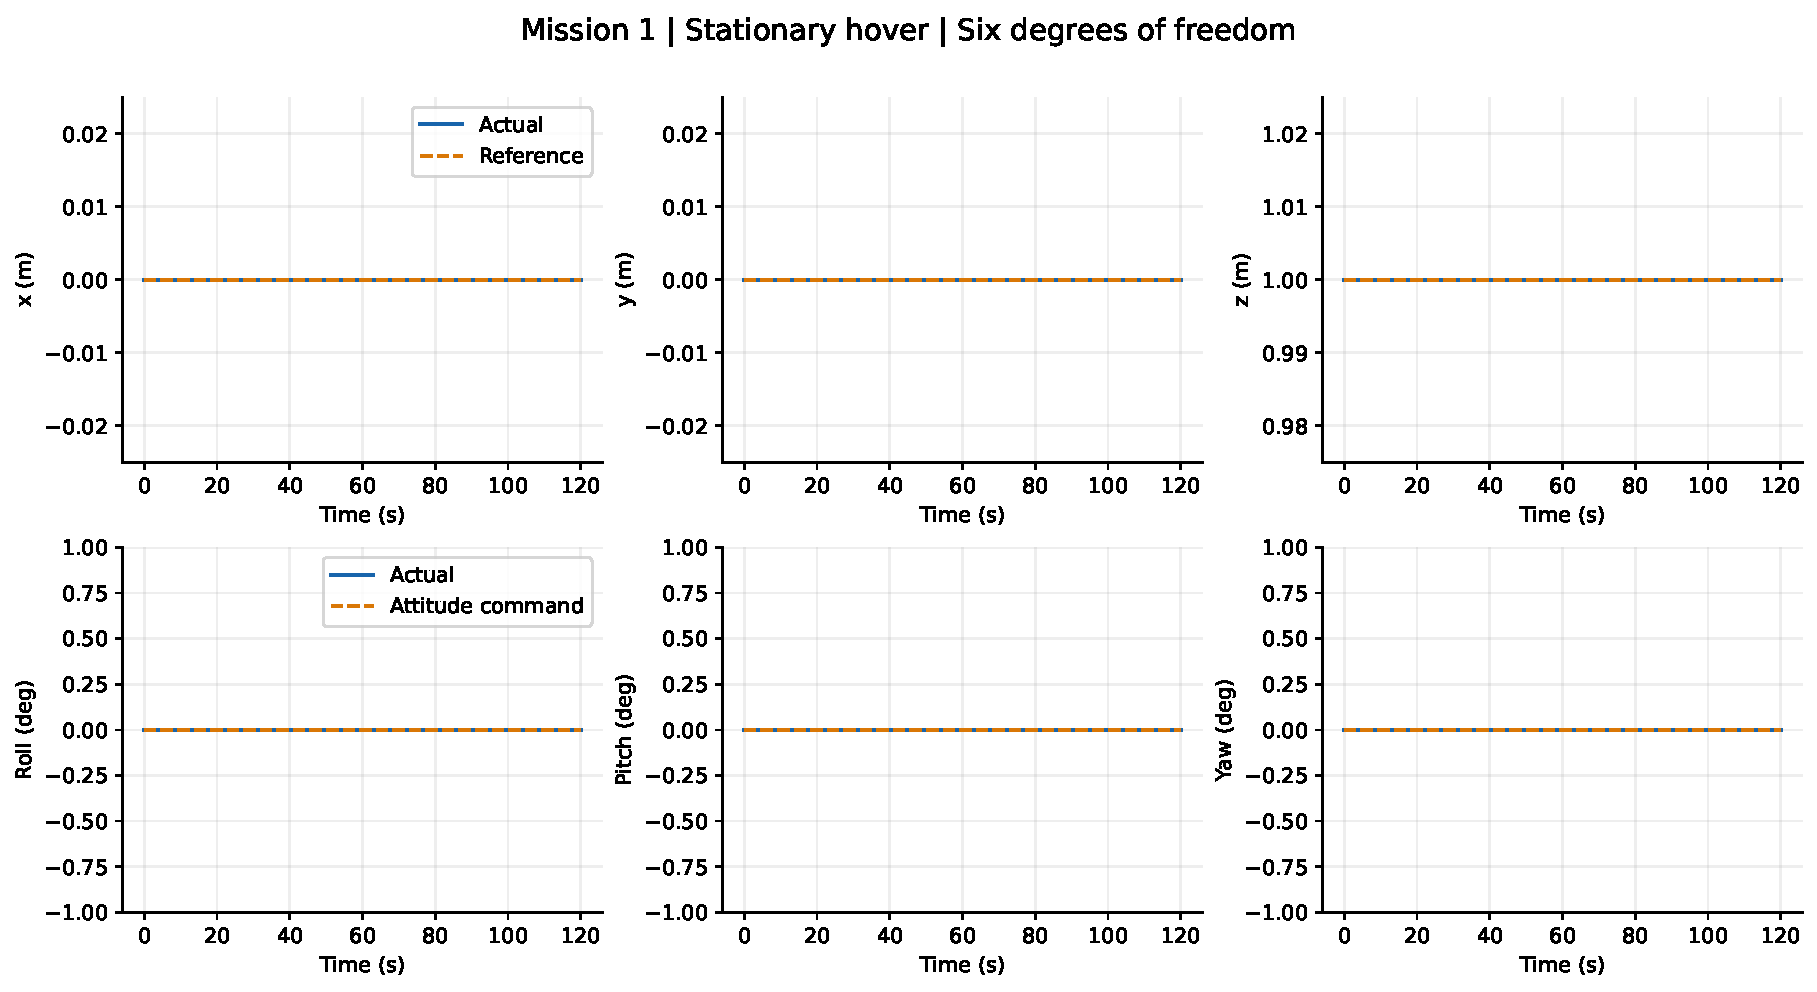
\includegraphics[width=\textwidth]{outputs/figures/hover_six_dof.pdf}
\caption{Hover: Position and Euler angles versus time. Solid curves are simulated states; dashed curves are references or attitude commands.}
\label{fig:hover-six_dof}
\end{figure}
\begin{figure}[htbp]
\centering
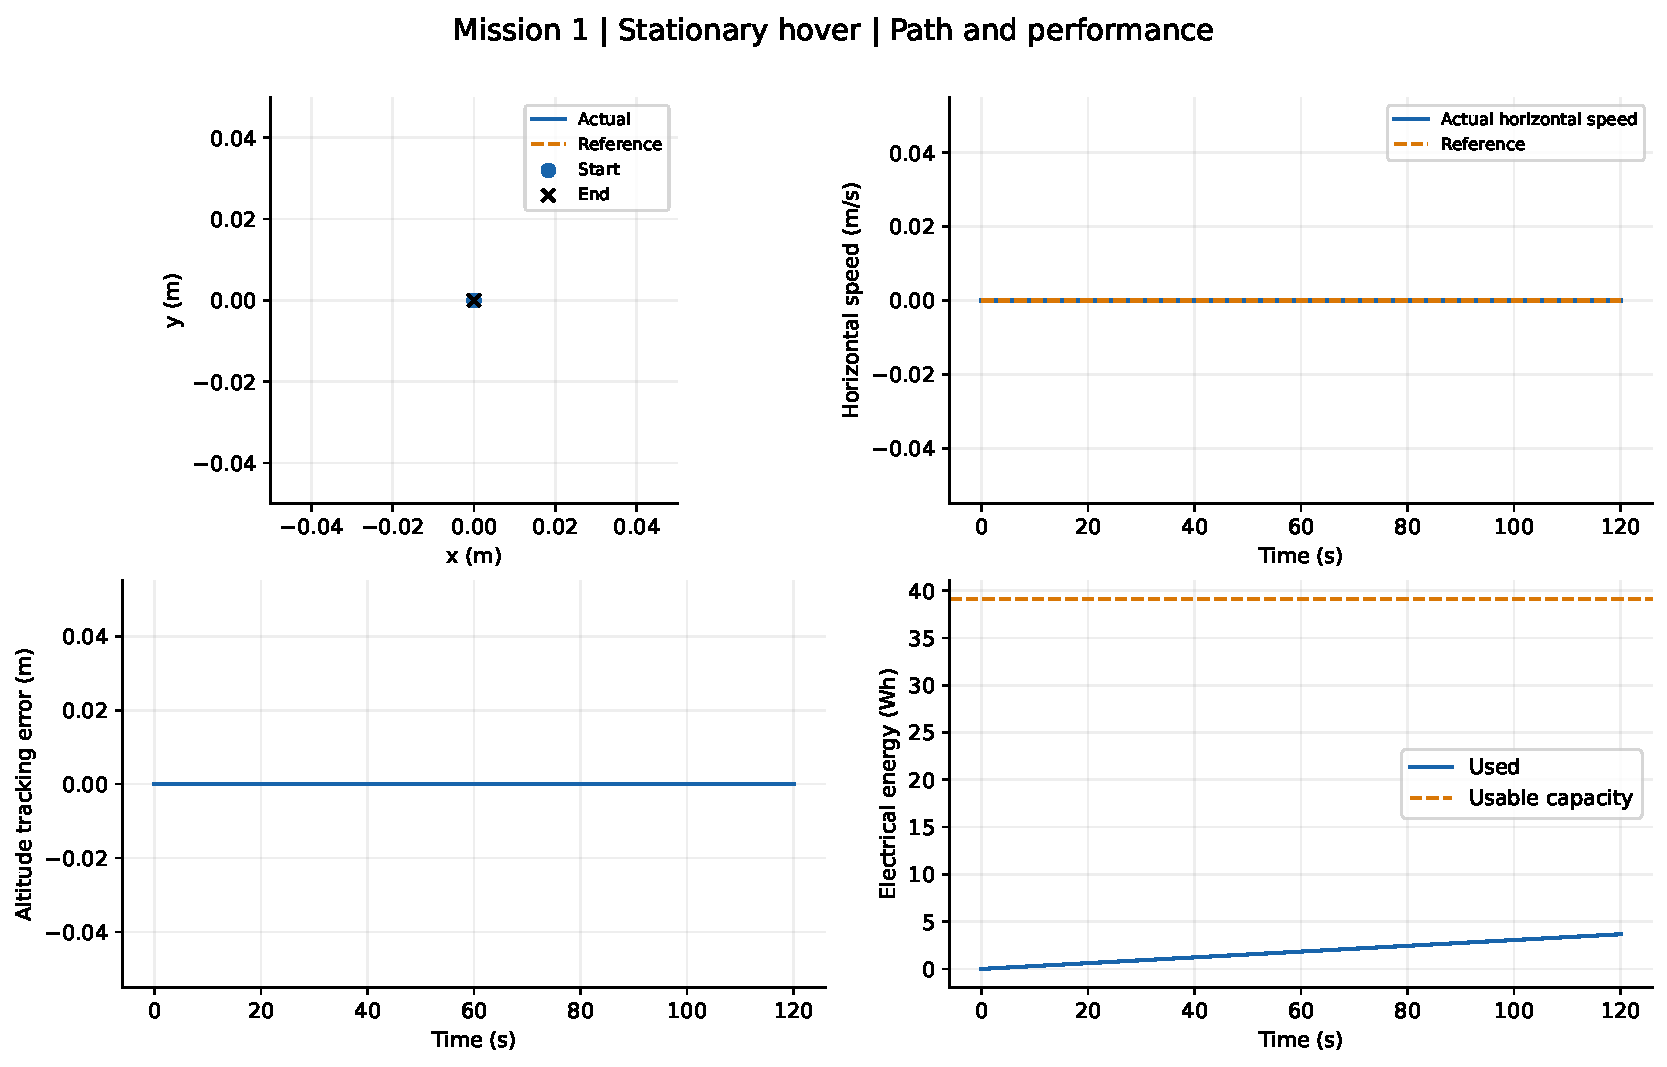
\includegraphics[width=\textwidth]{outputs/figures/hover_performance.pdf}
\caption{Hover: Actual and reference paths, horizontal speed, tracking error, and consumed electrical energy.}
\label{fig:hover-performance}
\end{figure}
\begin{figure}[htbp]
\centering
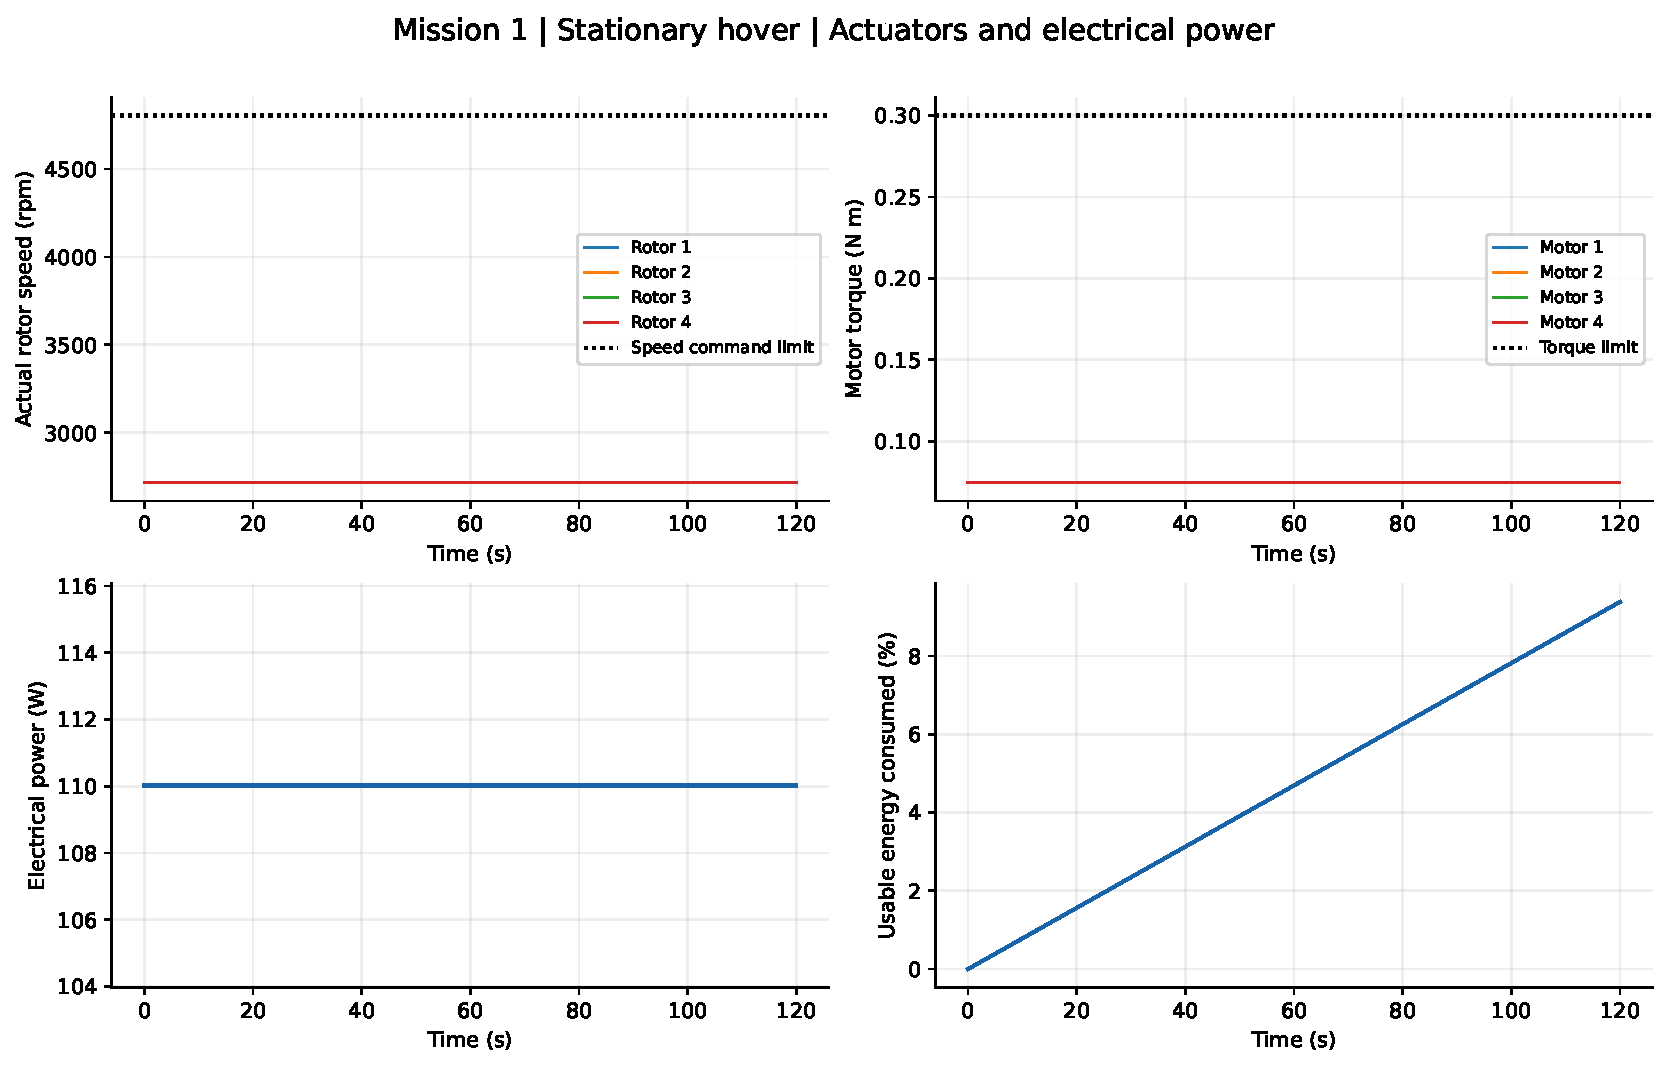
\includegraphics[width=\textwidth]{outputs/figures/hover_actuators.pdf}
\caption{Hover: Actual rotor speeds, applied motor torques, electrical power, and consumed fraction of usable battery energy.}
\label{fig:hover-actuators}
\end{figure}
\begin{figure}[htbp]
\centering
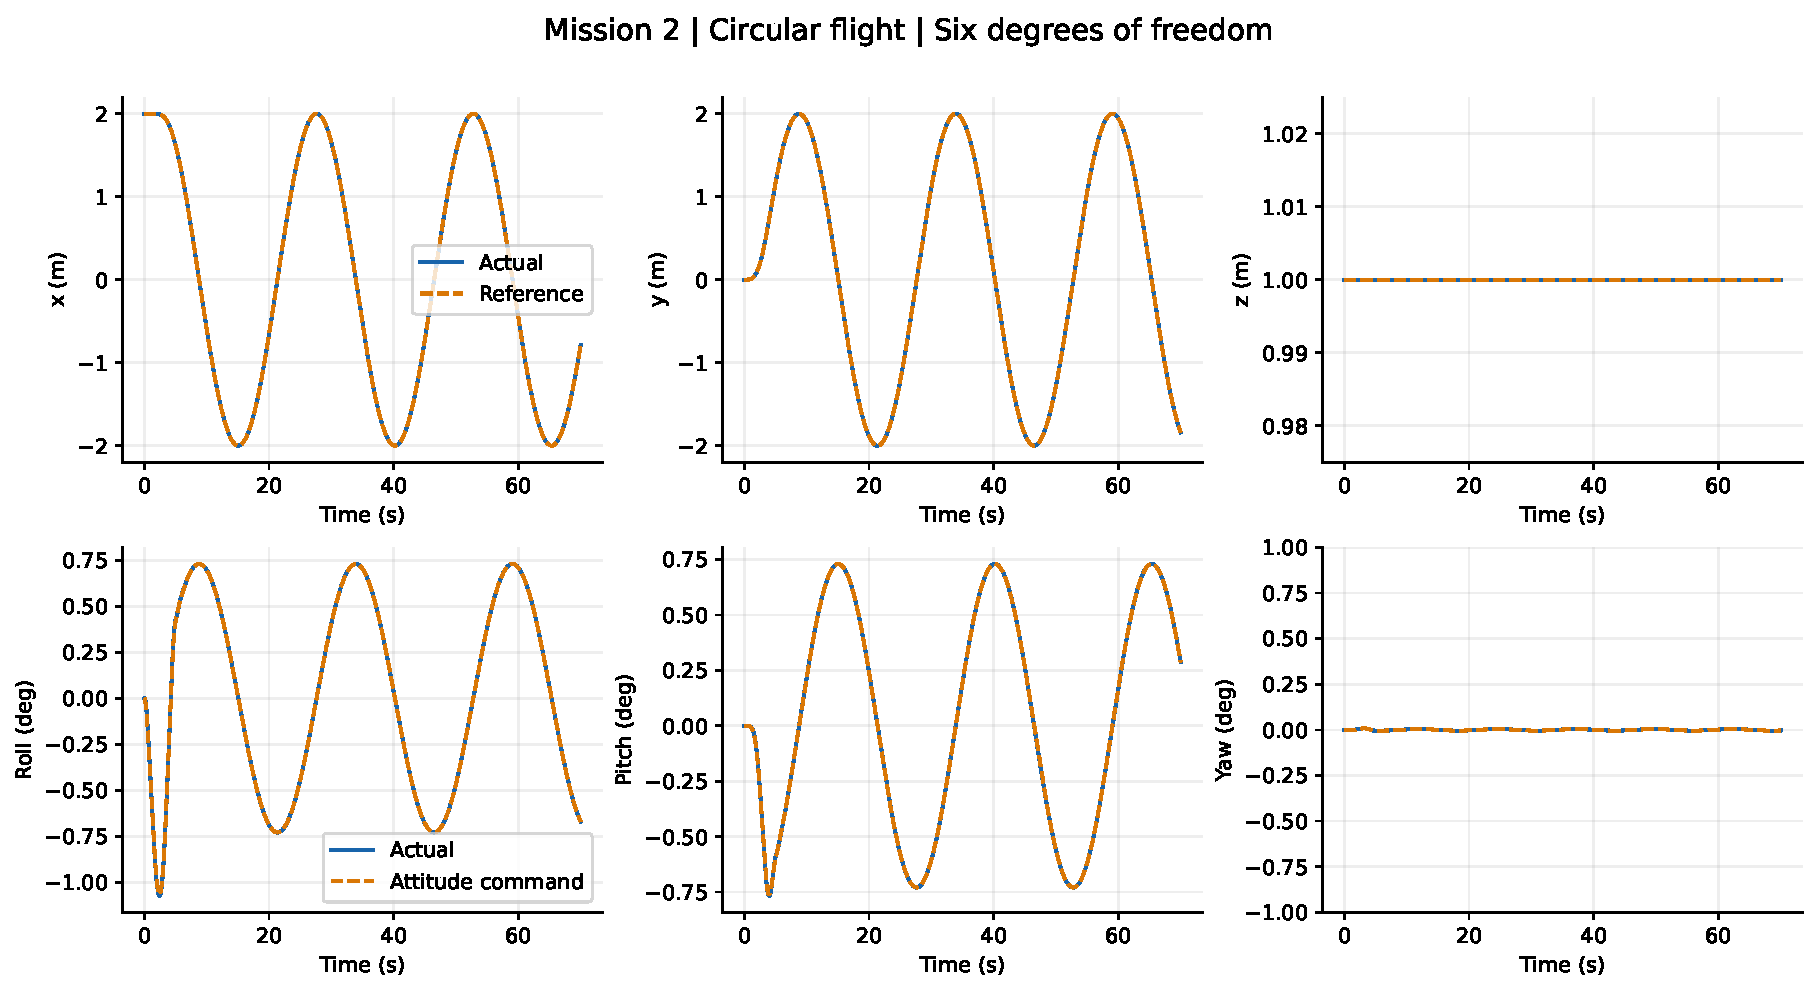
\includegraphics[width=\textwidth]{outputs/figures/circle_six_dof.pdf}
\caption{Circle: Position and Euler angles versus time. Solid curves are simulated states; dashed curves are references or attitude commands.}
\label{fig:circle-six_dof}
\end{figure}
\begin{figure}[htbp]
\centering
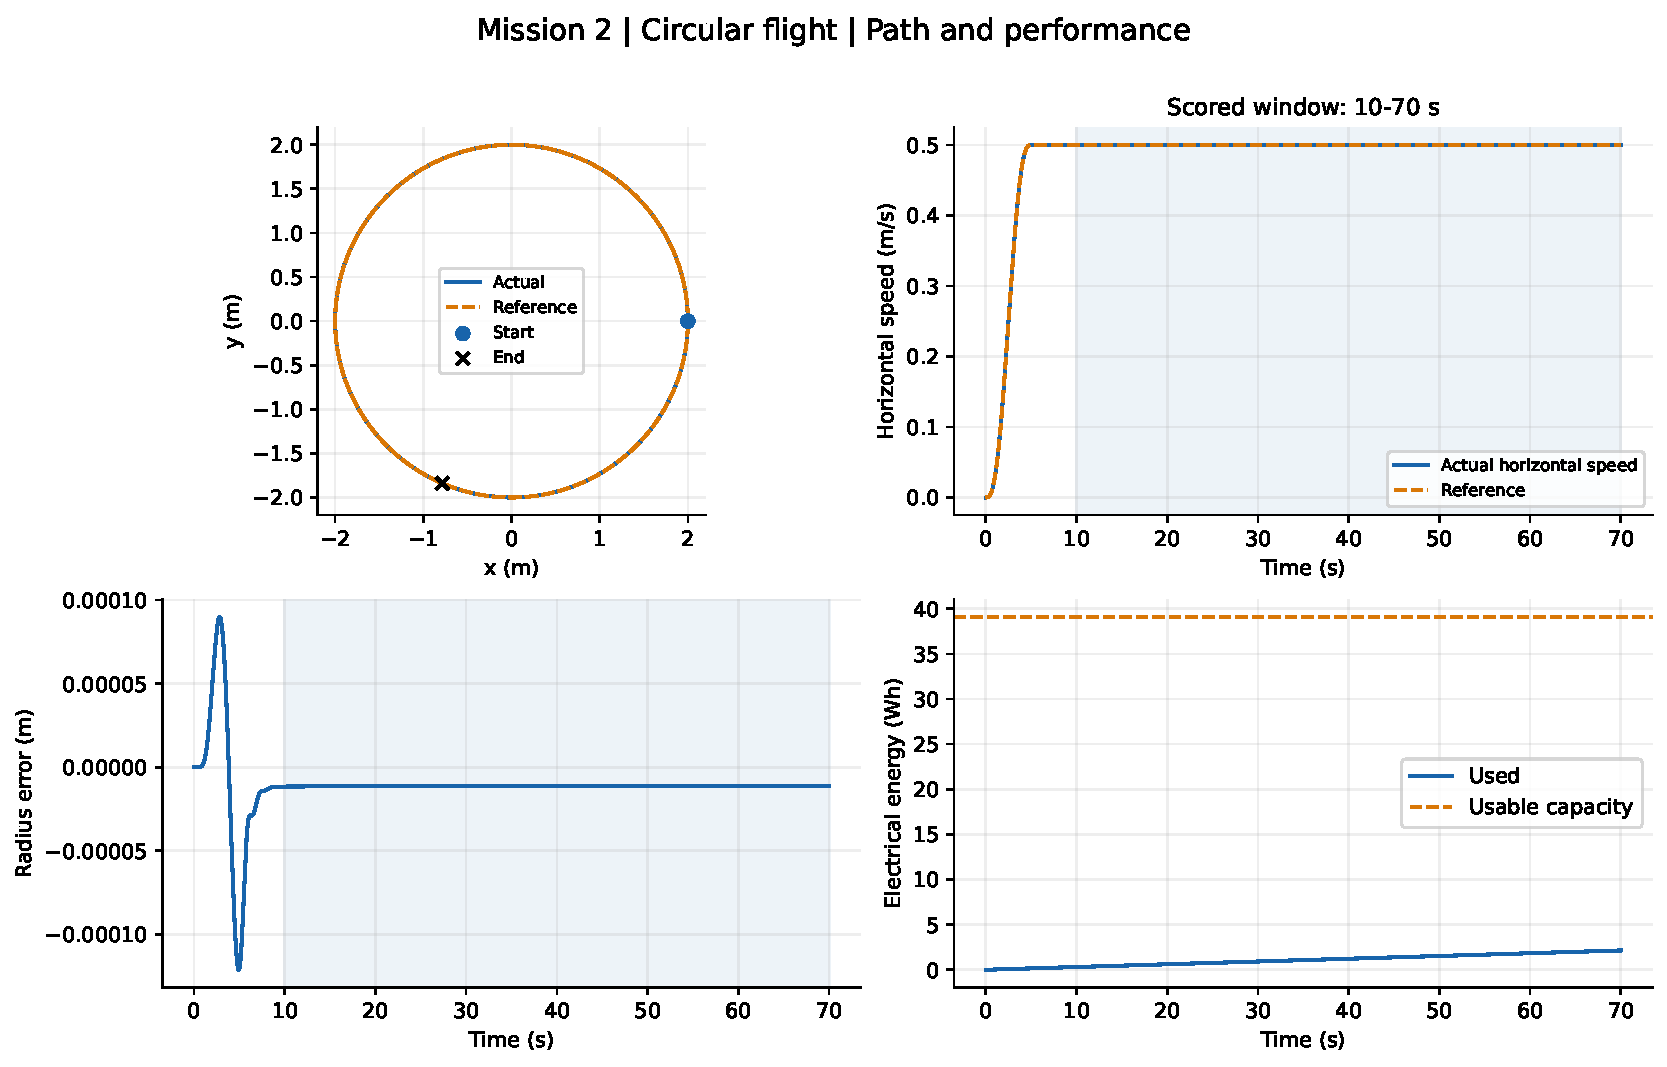
\includegraphics[width=\textwidth]{outputs/figures/circle_performance.pdf}
\caption{Circle: Actual and reference paths, horizontal speed, tracking error, and consumed electrical energy.}
\label{fig:circle-performance}
\end{figure}
\begin{figure}[htbp]
\centering
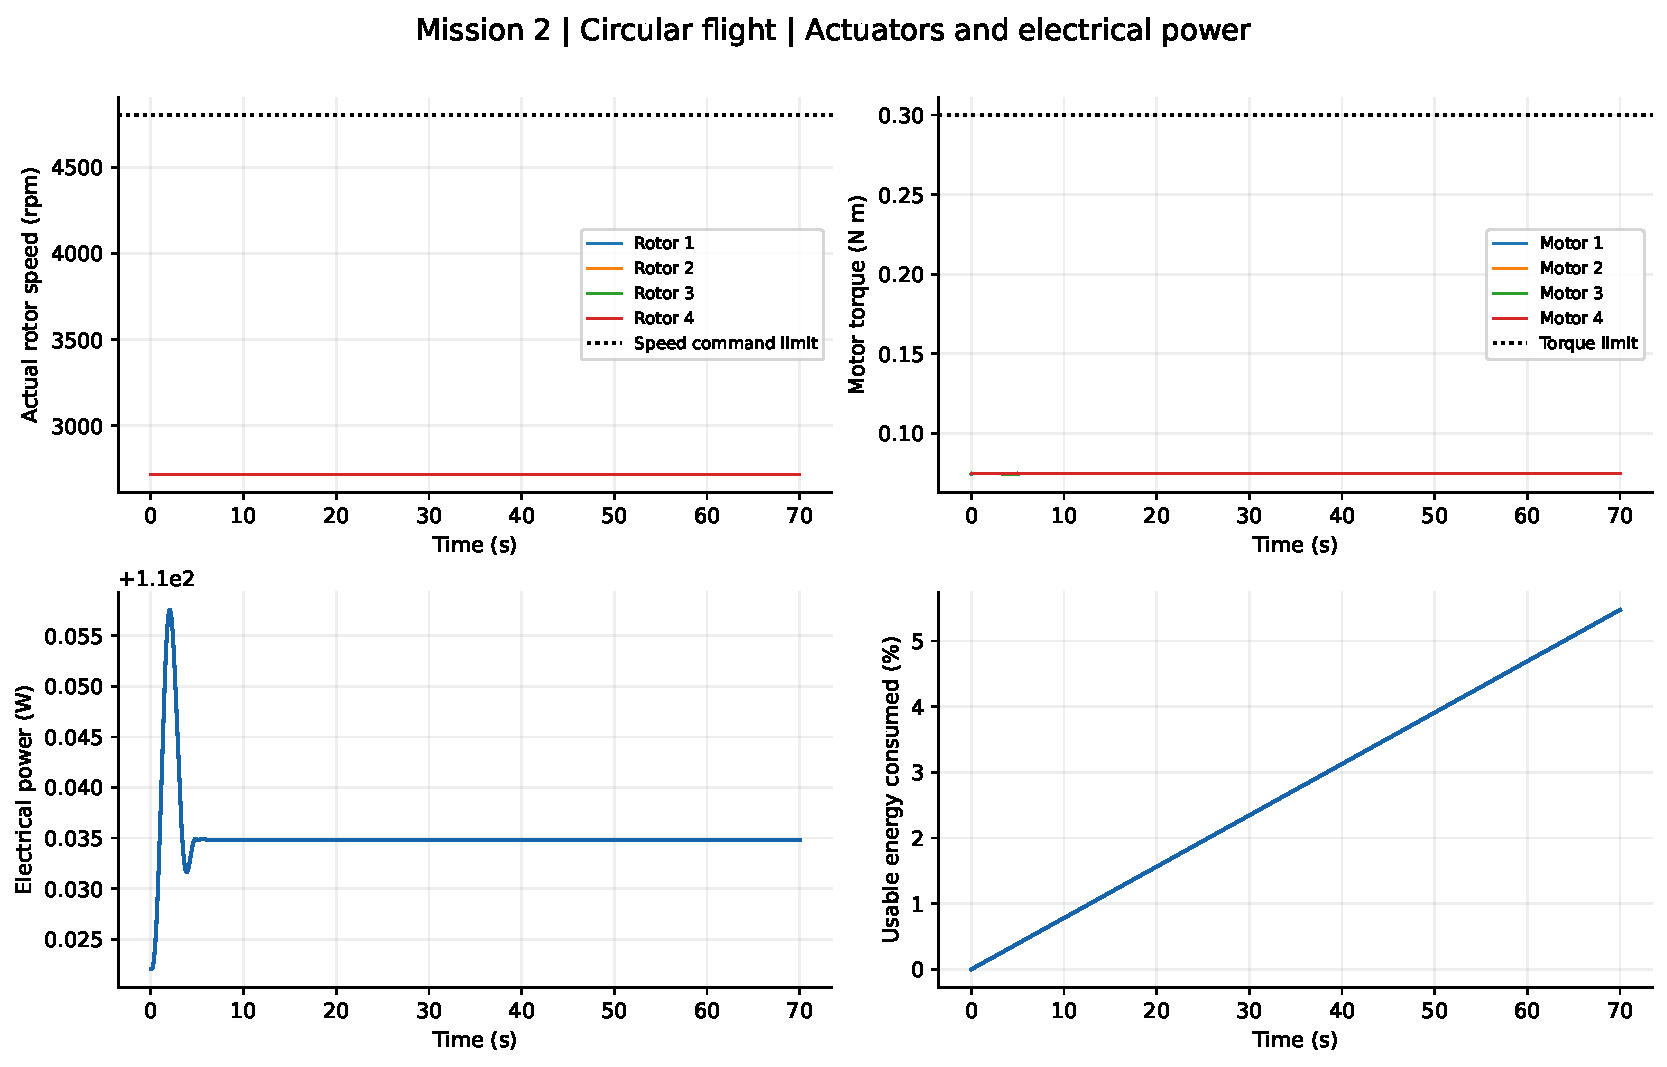
\includegraphics[width=\textwidth]{outputs/figures/circle_actuators.pdf}
\caption{Circle: Actual rotor speeds, applied motor torques, electrical power, and consumed fraction of usable battery energy.}
\label{fig:circle-actuators}
\end{figure}
\begin{figure}[htbp]
\centering
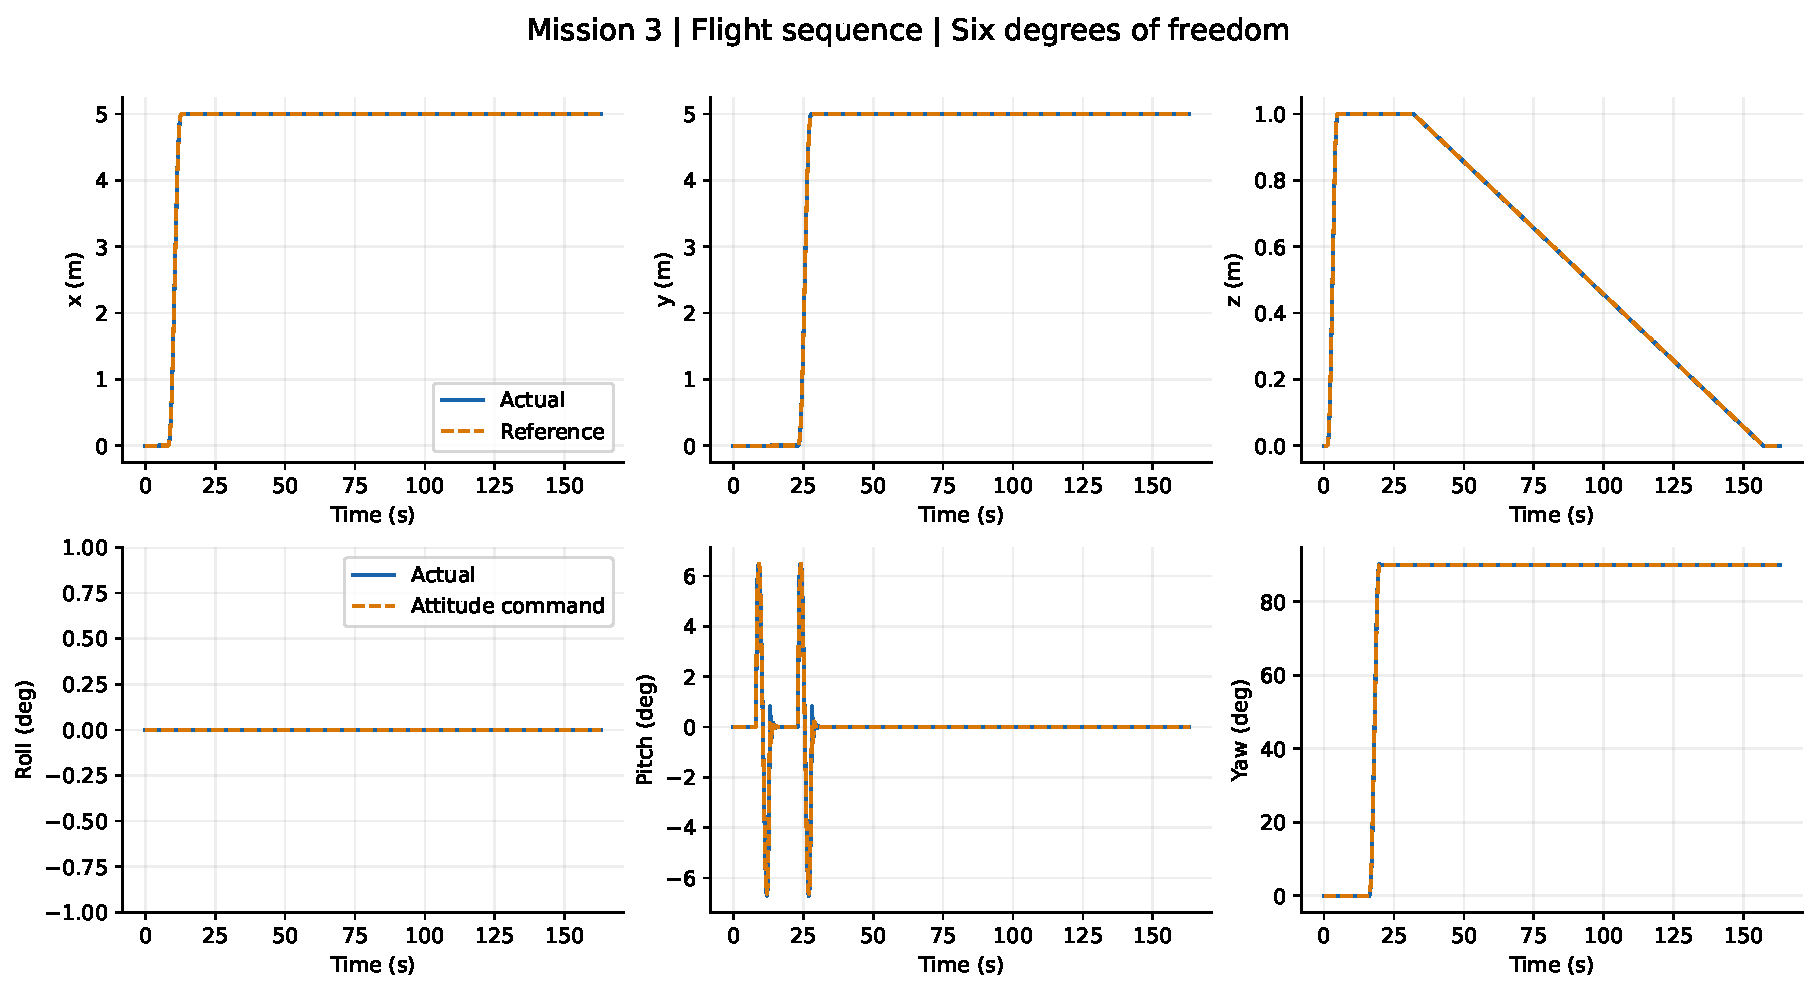
\includegraphics[width=\textwidth]{outputs/figures/sequence_six_dof.pdf}
\caption{Sequence: Position and Euler angles versus time. Solid curves are simulated states; dashed curves are references or attitude commands.}
\label{fig:sequence-six_dof}
\end{figure}
\begin{figure}[htbp]
\centering
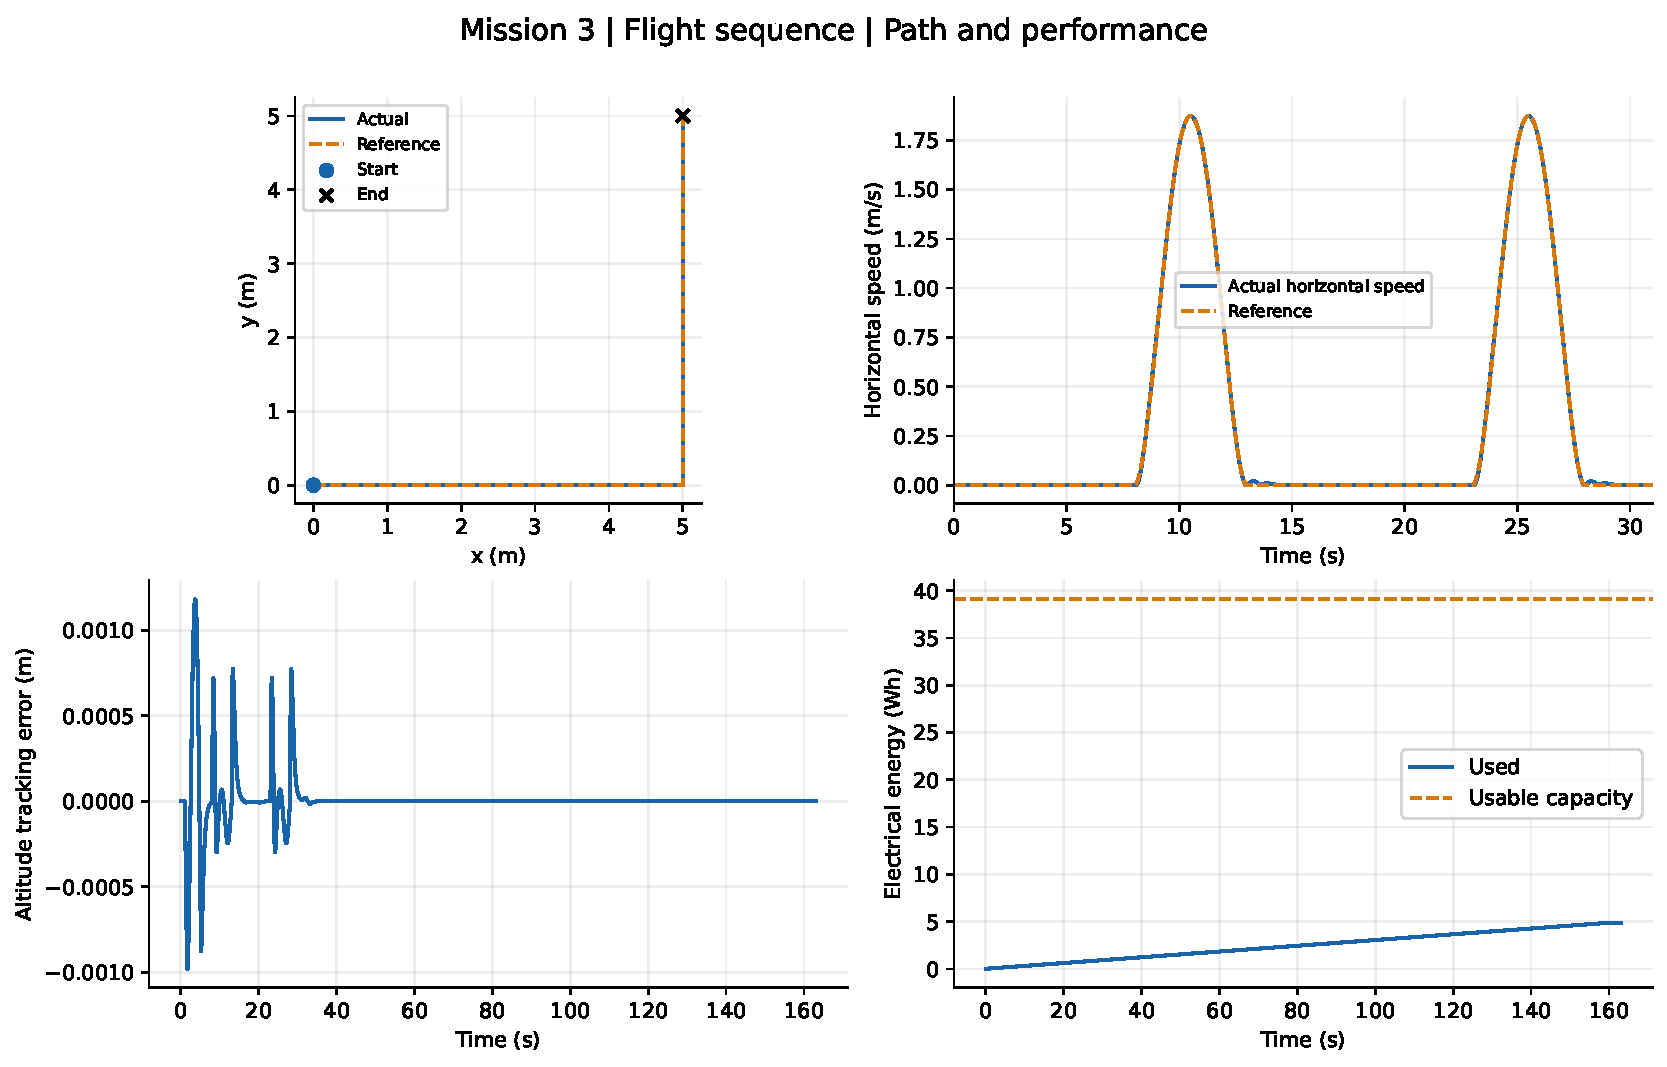
\includegraphics[width=\textwidth]{outputs/figures/sequence_performance.pdf}
\caption{Sequence: Actual and reference paths, horizontal speed, tracking error, and consumed electrical energy.}
\label{fig:sequence-performance}
\end{figure}
\begin{figure}[htbp]
\centering
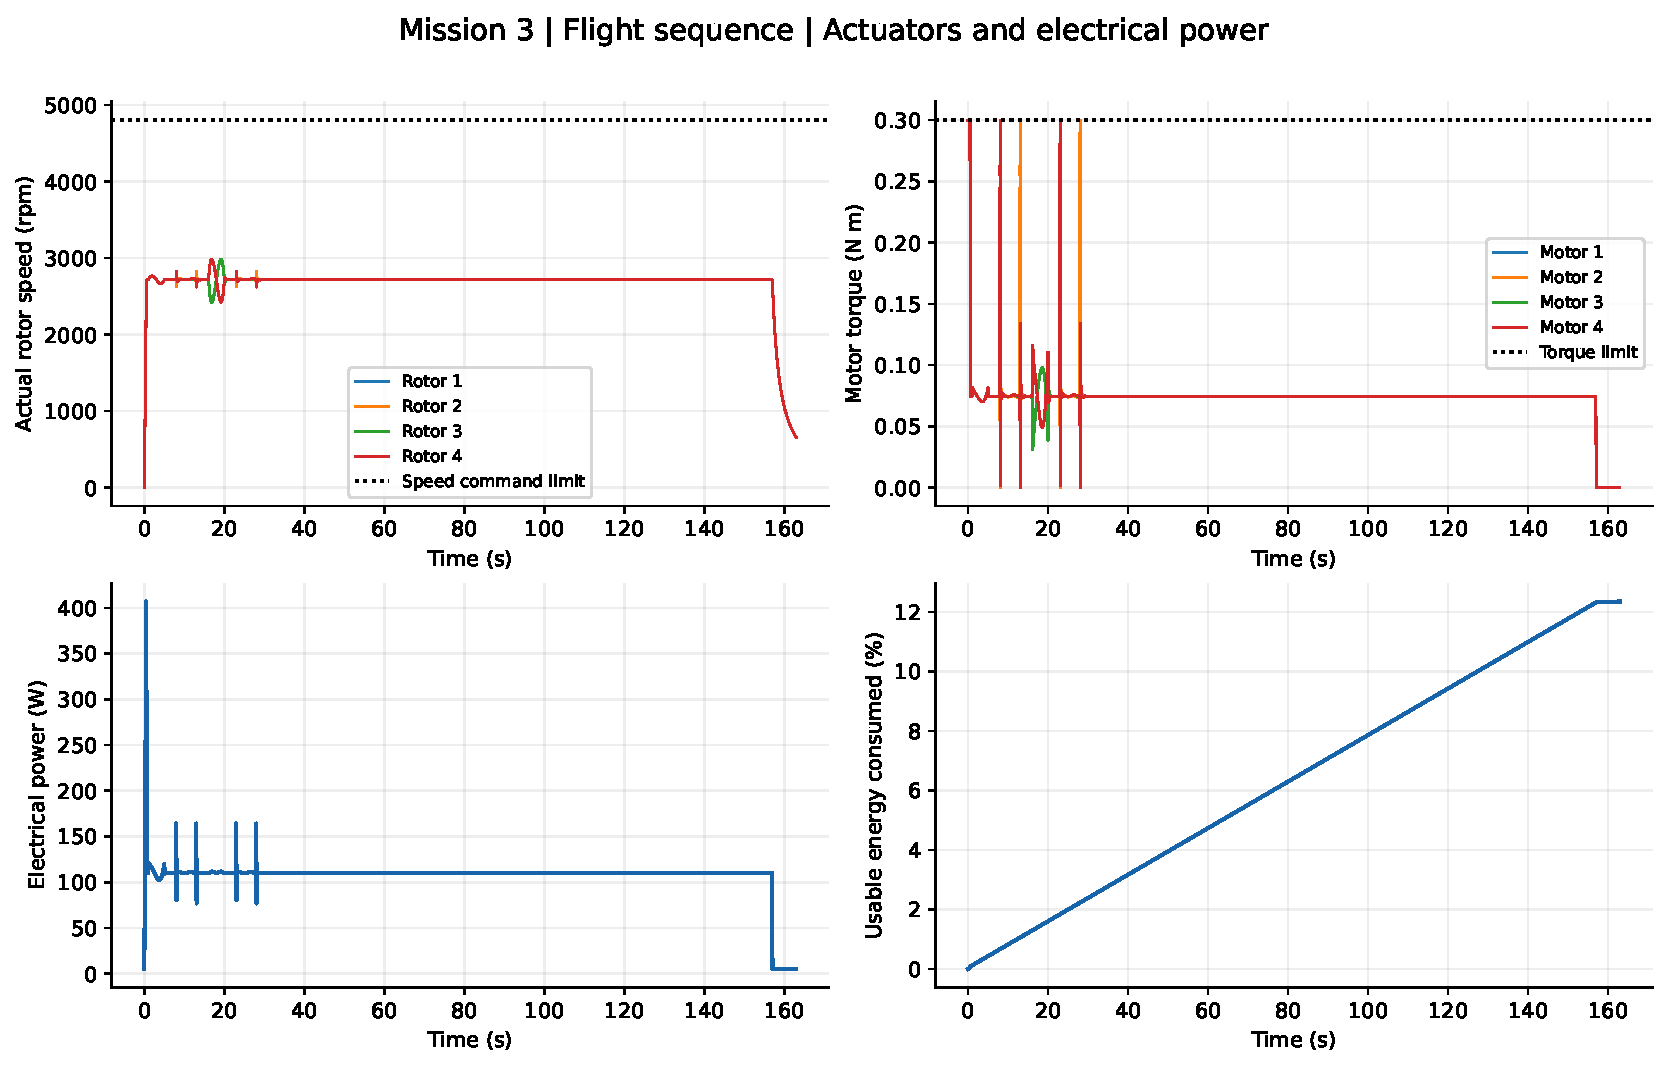
\includegraphics[width=\textwidth]{outputs/figures/sequence_actuators.pdf}
\caption{Sequence: Actual rotor speeds, applied motor torques, electrical power, and consumed fraction of usable battery energy.}
\label{fig:sequence-actuators}
\end{figure}
\begin{figure}[htbp]
\centering
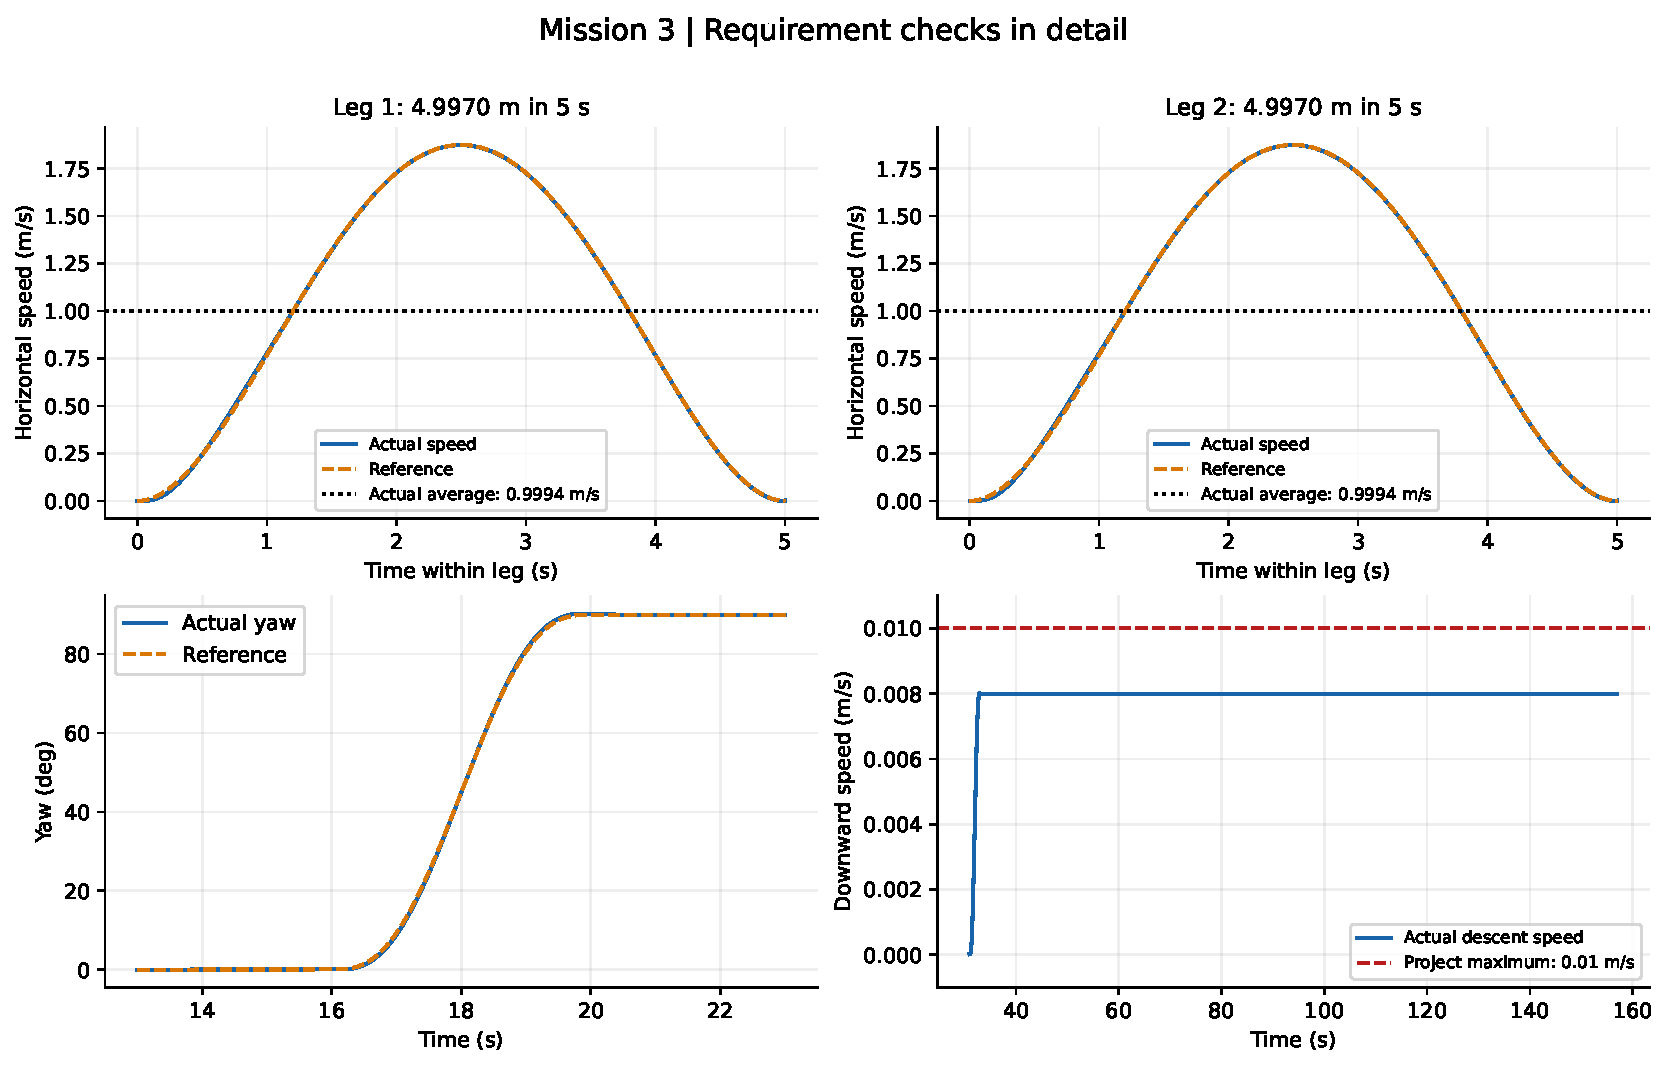
\includegraphics[width=\textwidth]{outputs/figures/sequence_detail.pdf}
\caption{Sequence: Straight-leg speeds and measured averages, left yaw maneuver, and descent-speed limit.}
\label{fig:sequence-detail}
\end{figure}